%%%%%%%%%%%%%%%%%%%%%%%%%%%%%%%%%%%%%%%%%
% FRI Data Science_report LaTeX Template
% Version 1.0 (28/1/2020)
% 
% Jure Demšar (jure.demsar@fri.uni-lj.si)
%
% Based on MicromouseSymp article template by:
% Mathias Legrand (legrand.mathias@gmail.com) 
% With extensive modifications by:
% Antonio Valente (antonio.luis.valente@gmail.com)
%
% License:
% CC BY-NC-SA 3.0 (http://creativecommons.org/licenses/by-nc-sa/3.0/)
%
%%%%%%%%%%%%%%%%%%%%%%%%%%%%%%%%%%%%%%%%%


%----------------------------------------------------------------------------------------
%  PACKAGES AND OTHER DOCUMENT CONFIGURATIONS
%----------------------------------------------------------------------------------------
\documentclass[fleqn,oneauthor,9pt]{ds_report}
\usepackage[english]{babel}

\graphicspath{{fig/}}


%----------------------------------------------------------------------------------------
%  ARTICLE INFORMATION
%----------------------------------------------------------------------------------------

% Header
\HWInfo{Bayesian Statistics Homework 1}

% Authors
\Authors{John Doe}

%----------------------------------------------------------------------------------------

\begin{document}

% Makes all text pages the same height
\flushbottom 

% Print the title and abstract box
\maketitle


%----------------------------------------------------------------------------------------
%  ARTICLE CONTENTS
%----------------------------------------------------------------------------------------

\section*{Introduction}
This is a compact version of the DS@FRI report template. It is intended for shorter reports, such as homeworks. It uses a smaller font, smaller margins and does not include the abstract.


%------------------------------------------------

\section*{Methods}

Use the Methods section to describe what you did an how you did it -- in what way did you prepare the data, what algorithms did you use, how did you test various solutions ... Provide all the required details for a reproduction of your work.

Below are examples of some common elements that you will probably need when writing your report (e.g. figures, equations, lists, code examples ...).


\subsection*{Equations}

You can write equations inline, e.g. $\cos\pi=-1$, $E = m \cdot c^2$ and $\alpha$, or you can include them as separate objects. The Bayes’s rule is stated mathematically as:

\begin{equation}
  P(A|B) = \frac{P(B|A)P(A)}{P(B)},
  \label{eq:bayes}
\end{equation}
where $A$ and $B$ are some events. You can also reference it -- the equation \ref{eq:bayes} describes the Bayes's rule.

\subsection*{Figures}

You can insert figures, for example \figurename~\ref{fig:column}.

\begin{figure}[ht]\centering
  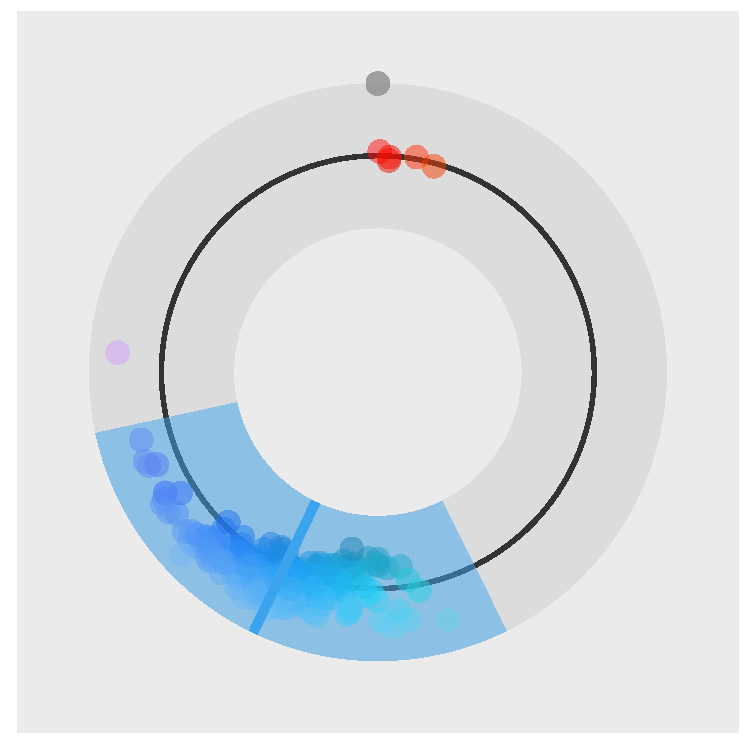
\includegraphics[width=\linewidth]{figure_example.pdf}
  \caption{\textbf{A random visualization.} This is an example figure.}
  \label{fig:column}
\end{figure}

\subsection*{Code examples}

You can also insert short code examples. You can specify them manually, or insert a whole file with code. Please avoid inserting long code snippets, advisors will have access to your repositories and can take a look at your code there. If necessary, you can use this technique to insert code (or pseudo code) of short algorithms that are crucial for the understanding of the manuscript.

\lstset{language=Python}
\lstset{caption={Insert code directly from a file.}}
\lstset{label={lst:code_file}}
\lstinputlisting[language=Python]{code/example.py}

\lstset{language=R}
\lstset{caption={Write the code you want to insert.}}
\lstset{label={lst:code_direct}}
\begin{lstlisting}
import(dplyr)
import(ggplot)

ggplot(diamonds,
     aes(x=carat, y=price, color=cut)) +
  geom_point() +
  geom_smooth()
\end{lstlisting}


\subsection*{Tables}

Use the table environment to insert tables.

\begin{table}[hbt]
  \caption{Table of grades.}
  \centering
  \begin{tabular}{l l | r}
    \toprule
    \multicolumn{2}{c}{Name} \\
    \cmidrule(r){1-2}
    First name & Last Name & Grade \\
    \midrule
    John & Doe & $7.5$ \\
    Jane & Doe & $10$ \\
    Mike & Smith & $8$ \\
    \bottomrule
  \end{tabular}
  \label{tab:label}
\end{table}

%------------------------------------------------

\section*{Results}

Use the results section to present the final results of your work. Present the results in a objective and scientific fashion. Use visualisations to convey your results in a clear and efficient manner. When comparing results between various techniques use appropriate statistical methodology.

%------------------------------------------------

\section*{Discussion}

Use the Discussion section to objectively evaluate your work, do not just put praise on everything you did, be critical and exposes flaws and weaknesses of your solution. You can also explain what you would do differently if you would be able to start again and what upgrades could be done on the project in the future.

\end{document}
